\documentclass[12pt,a4paper]{article}

\usepackage[utf8]{inputenc}
\usepackage[russian]{babel}
\usepackage[OT1]{fontenc}
\usepackage{amsmath}
\usepackage{amsfonts}
\usepackage{amssymb}
\usepackage{graphicx}
\usepackage{tikz}
\usepackage{pgfplots}
\usepackage[export]{adjustbox}
\usepackage{wrapfig}
\usepackage[left=2cm,right=2cm,top=2cm,bottom=2cm]{geometry}
\usepackage{setspace}


\begin{document}

\title{
2.1.3.

Определение $C_p/C_v$ по скорости звука в газе.
\author{Семёнов Андрей Б02-016}
}
\date{14 апреляля 2021г.}

\maketitle

\newpage


\textbf{Цель работы:} Измерение частоты колебаний и длины волны при резонансе звуковых колебаний в газе, заполняющем трубу

\textbf{В работе используются:} звуковой генератор ГЗ, электронный осциллограф ЭО, микрофон, телефон, раздвижная труба, теплоизолированная труба, обогреваемая водой из термостата, баллон со сжатым углекислым газом, газгольдер.

\section{Теоретические сведения.}
Из теории нам известна зависимость скорости звука от показателя адиабаты $\gamma$:
$$c = \sqrt{\gamma\frac{RT}{\mu}}.$$
Таким образом, задача нахождения $\gamma$ сходится к задаче нахождения скорости звука при заданной температуре.\\
В этом эксперименте предпологается использовать стоячие волны для нахождения $c$. Известно, что стоячие волны в коридоре длиной $L$ образуются при:
$$L = \frac{n}{2}\lambda,$$
где $\lambda$ -- длина волны звука, связанная со скоростью звука и частотой $f$, как:
$$\lambda = c/f.$$
То есть верно, что:
$$L = \frac{c}{2f}n.$$
В текущем эксперименте мы будем знать не абсолютный номер порядка $n$, а его приращение $k = n - n_0$, для которого верно, что:
$$\Delta L = L - L_0 = \frac{c}{2f}k + \Delta L_0,$$
где $L_0$ -- минимальный размер трубы, а $\Delta L$ -- отклонение от него, которое мы можем измерить.



\section{Экспериментальная установка}
В этой работе мы будем измерять зависимость $\Delta L(k)$ при постоянных значениях $f$, из чего получим $c$. Для этого мы используем установку на Рис. 1. Эта установка представляет из себя две вложенных друг в друга трубы с миллиметровой шкалой на подвижной части. На краях этой системы установлены приемник Т и передатчик М. Также к системе подведена трубка, через которую можно накачивать пространство внутри труб воздухом или углекислым газом.
\begin{center}
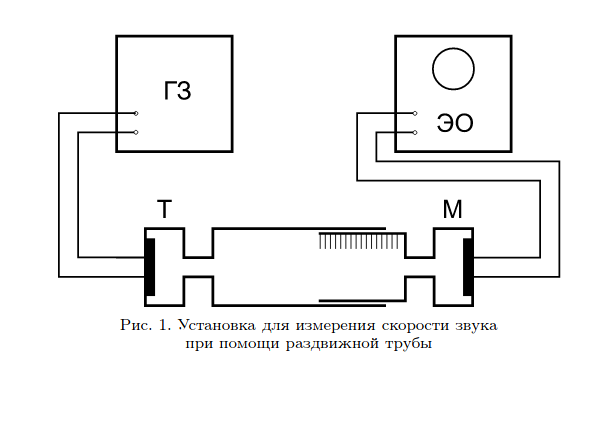
\includegraphics[width=0.95\textwidth]{equip.png}.
\end{center}


\section{Выполнение работы.}


\end{document}